\documentclass[10pt,a4paper]{article}
\usepackage[utf8]{inputenc}
\usepackage{amsmath}
\usepackage{amsfonts}
\usepackage{amssymb}
\setlength{\parindent}{0pt}
\usepackage{subcaption}
\usepackage{graphicx}
\usepackage{listings}
\usepackage{lastpage}
\usepackage{color} %red, green, blue, yellow, cyan, magenta, black, white
\definecolor{mygreen}{RGB}{28,172,0} % color values Red, Green, Blue
\definecolor{mylilas}{RGB}{170,55,241}
\usepackage{breqn}
\usepackage{float}
\usepackage{fancyhdr}
\usepackage{cancel}
\usepackage{enumitem}
\usepackage{placeins}
\pagestyle{fancy}
\usepackage{titling}
\usepackage{units}
\usepackage{forest}
\usepackage{hyperref}

\newcommand{\subtitle}[1]{%
	\posttitle{%
		\par\end{center}
	\begin{center}\large#1\end{center}
	\vskip0.5em}%
}


\lhead{ENAE685 Final Project}
\rhead{Kennedy}

\title{ENAE685 Final Project}
\subtitle{Solving the 2-D Navier-Stokes Equations}
\author{Matt Kennedy}

\cfoot{\thepage\ of \pageref{LastPage}}

\begin{document}


\lstset{language=Matlab,%
	%basicstyle=\color{red},
	breaklines=true,%
	morekeywords={matlab2tikz},
	keywordstyle=\color{blue},%
	morekeywords=[2]{1}, keywordstyle=[2]{\color{black}},
	identifierstyle=\color{black},%
	stringstyle=\color{mylilas},
	commentstyle=\color{mygreen},%
	showstringspaces=false,%without this there will be a symbol in the places where there is a space
	numbers=left,%
	numberstyle={\tiny \color{black}},% size of the numbers
	numbersep=9pt, % this defines how far the numbers are from the text
	emph=[1]{for,end,break},emphstyle=[1]\color{red}, %some words to emphasise
	%emph=[2]{word1,word2}, emphstyle=[2]{style},    
}

\lstdefinestyle{CStyle}{
    backgroundcolor=\color{backgroundColour},   
    commentstyle=\color{mGreen},
    keywordstyle=\color{magenta},
    numberstyle=\tiny\color{mGray},
    stringstyle=\color{mPurple},
    basicstyle=\footnotesize,
    breakatwhitespace=false,         
    breaklines=true,                 
    captionpos=b,                    
    keepspaces=true,                 
    numbers=left,                    
    numbersep=5pt,                  
    showspaces=false,                
    showstringspaces=false,
    showtabs=false,                  
    tabsize=2,
    language=C
}



\begin{minipage}[h]{\textwidth}
	\maketitle
	
\end{minipage}



%\begin{center}
%\huge{ENAE685 Homework \#7}
%\large{1-D Shock Tube: Subsonic, Transonic (Explicit in Time)}
%\large{Chris Thurman\\ Matt Kennedy \\ Nicole Anderson}
%\end{center}

\vspace{12cm}

\section*{ABSTRACT}


%The following homework presents a numerical solution to the 1-D shock tube problem using unsteady Euler equations. Van-Leer Flux Vector Splitting was implemented to examine Sod's problem (subsonic flow,) Lax's problem (supersonic flow,) and Lax's problem with reflective boundary conditions. The exact solution for each case was also calculated for error comparison and a grid refinement study was performed.

In this project the Navier-Stokes equations are solved for compressible flow, including shear stresses and heat fluxes to the previously solved Euler Equations. The solutions are applied to a flat plate in a supersonic flow at varying incident angles, as well as Couette flow with varying pressure gradients. Solvers are developed in both MATLAB and CUDA C.


\thispagestyle{empty} % supress the page number and headers

\newpage

\setcounter{page}{1}


\section*{TOPIC OVERVIEW}
%While my original topic was set out to be analysis of flow in a 2-D rocket nozzle, I found that there were few CFD problems I was capable of solving and were actually interesting. Insteady, as more of a challenge, I turned to solving the Navier-Stokes equations over a flat plate and explored several applications. Unfortunately due to technical difficulties I was unable to port the MATLAB code over to CUDA, however it was still written in a non-vectorized format to assist in porting at a later time.

While I initially set out to explore 2-D flow through a nozzle, I had trouble finding interesting ways to expand the analysis and instead turned my interest to solving the full Navier-Stokes equations. After some initial troubles getting the CUDA compiler to install on an old Linux machine, I did finally get a working version of the base case (flow over top of thin flat plate) working in CUDA. The CUDA version runs only moderately faster than the MATLAB version, however further optimizations can be done and I expect that the CUDA version will scale much better as the grid size is increased from 70x70. All plots and analysis in this report were generated with the MATLAB version, although the same results are expected with trivial changes to the CUDA version.


%Unfortunately due to technical difficulties I was unable to port the MATLAB code over to CUDA (installing the CUDA development kit on an old Linux system that already has drivers is a conflict nightmare,) however the MATLAB was still written in a non-vectorized format to assist in replication to C/CUDA at a later time.

\section*{THEORY}


For this project the 2-D Navier-Stokes are solved for compressible flow, integrating shear stresses and heat fluxes to the previously solved Euler Equations. The 2-D Navier-Stokes equations in their conservative form are:\\


% just give all the equations here?

\textbf{Continuity:}

\begin{align*}
\frac{\partial \rho}{\partial t} + \frac{\partial}{\partial x}(\rho u) + \frac{\partial }{\partial y} (\partial v) = 0
\end{align*}

\textbf{x-Momentum:}

\begin{align*}
\frac{\partial}{\partial t}(\rho u) + \frac{\partial}{\partial x} (\rho u^2 + p - \tau_{xx}) + \frac{\partial}{\partial y} (\rho u v - \tau_{xy}) = 0
\end{align*}

\textbf{y-Momentum:}

\begin{align*}
\frac{\partial}{\partial t}(\rho v) + \frac{\partial}{\partial x} (\rho u v - \tau_{xy}) + \frac{\partial}{\partial y} (\rho  v^2 + p - \tau_{yy}) = 0
\end{align*}


\textbf{Energy:}

\begin{align*}
\frac{\partial}{\partial t}(E_t) + \frac{\partial }{\partial x}[(E_t + p) u + q_x - u \tau_{xx} - v \tau_{xy}] + \frac{\partial}{\partial y}[(E_t + p)v + q_y - u \tau_{yx} - v \tau_{yy}] = 0
\end{align*}


Where $E_t$ is the sum of kinetic and internal energy,

\begin{align*}
E_t = \rho e + \frac{1}{2} \rho ( u^2 + v^2)
\end{align*}


The shear and normal stresses, $\tau_{xx}$, $\tau_{yy}$, $\tau_{xy}$:

\begin{align*}
\tau_{xy} = \mu \left( \frac{\partial u}{\partial y} + \frac{\partial v}{\partial x} \right)
\end{align*}

\begin{align*}
\tau_{xx} = \lambda \left( \frac{\partial u}{\partial x} + \frac{\partial v}{\partial y} \right) + 2 \mu \frac{\partial u}{\partial x}
\end{align*}

\begin{align*}
\tau_{yy} = \lambda \left( \frac{\partial u}{\partial x} + \frac{\partial v}{\partial y} \right) + 2 \mu \frac{\partial v}{\partial y}
\end{align*}

Where $\lambda$ is the second viscosity coefficient estimated by Stokes to be:

\begin{align*}
\lambda = -\frac{2}{3} \mu
\end{align*}

and, assuming a calorically perfect gas, Suutherland's law can be used to get the local $\mu$:

\begin{align*}
\mu = \mu_0 \left( \frac{T}{T_0} \right)^{3/2} \frac{T_0 + 110}{T + 110}
\end{align*}


The heat flux terms $q_x$ and $q_y$ can be determined from Fourier's law of thermal conduction which relates the thermal conductivity, $k$, and the temperature gradient:

\begin{align*}
q = -k \nabla T = \left( -k\frac{\partial T}{\partial x}, -k\frac{\partial T}{\partial y} \right)
\end{align*}

Thermal conductivity can be made a function of Temperature through assuming the Prandtl number is constant at $\approx 0.71$:

\begin{align*}
k(T) = \frac{\mu (T) c_p }{\text{Pr}}
\end{align*}






There are now two flux vectors, F and G, corresponding to the fluxes in the x- and y-directions, in addition to the conserved variable vector Q:

\begin{align*}
F = 
\begin{bmatrix} 
\rho u \\
\rho u^2 + p - \tau_{xx}\\
\rho u v - \tau_{xy}\\
(E_t + p) u - u \tau_{xx} - v \tau_{xy} + q_x
\end{bmatrix}
\end{align*}


\begin{align*}
G = 
\begin{bmatrix} 
\rho v \\
\rho u v - \tau_{xy}\\
\rho v^2 + p - \tau_{yy}\\
(E_t + p) v - u \tau_{xy} - v \tau_{yy} + q_y
\end{bmatrix}
\end{align*}


\begin{align*}
Q = 
\begin{bmatrix}
\rho \\
\rho u \\
\rho v \\
E_t
\end{bmatrix}
\end{align*}



For our cases, the gravity component of the Navier-Stokes has been ignored.\\





\section*{PROGRAM}

The MATLAB program consists of a main file, \textit{initialize.m}, ten functions which get called every iteration, and one function to calculate the analytical boundary layer thickness to assist in establishing an appropriate domain.\\

\textit{Chapter 10, Supersonic Flow over a Flat Plate: Numerical Solution by Solving the Complete Navier-Stokes Equations} from Anderson was loosly followed.\\

MacCormack's method was used as a simple but fairly robust iteration scheme for 2-D flow. Uniform grid spacing was also selected for simplicity sake, and while this limits the application cases to flow over flat plates or walls (rather than say, an airfoil,) this is still sufficient for initially exploring the Navier-Stokes solutions.\\

With the plan of porting this code over to CUDA C/C++ from the start, functions within the main iteration loop were designed to operation on a single point at a time such that $(JMAX*KMAX)$ threads could be launched and operate on each point independently.\\


The boundary condition application was separated into different functions because for cases where the wall goes all the way to $j=1$ or $j=JMAX$ on the left or right side, the inflow or outflow boundary needs to be evaluated prior to the wall values being updated with the inflow or outflow conditions. When all points are being evaluated simultaneously there is no way to enforce this order so it was split into two separate operations with the threads syncing in between.

\subsection*{Iteration Scheme:}

MacCormack's scheme was implemented as follows:

\begin{align*}
\text{Flux\_Predictor}_{j,k} & = \frac{\text{F}_{j+1,k} - \text{F}_{j,k}}{\Delta x} + \frac{ \text{G}_{j,k+1} - \text{G}{j,k} }{\Delta y} \\
\text{Q\_Predictor}_{j,k} & = \text{Q}_{j,k} - \Delta t (\text{Flux\_Predictor}_{j,k})
\end{align*}

F\_Predictor and G\_Predictor are then calculated from the values of Q\_Predictor.

\begin{align*}
\text{Flux}_{j,k} & = \frac{\text{F\_Predictor}_{j,k} - \text{F\_Predictor}_{j-1,k}}{\Delta x} + \frac{\text{G\_Predictor}_{j,k} - \text{G\_Predictor}_{j,k-1}}{\Delta y}\\
\text{Q}_{j,k} & = \frac{1}{2} \left[ \text{Q}_{j,k} + \text{Q\_Predictor}_{j,k} - \Delta t (\text{Flux}_{j,k}) \right]
\end{align*}


\subsection*{Time Step:}

Per Anderson, the time step size was defined as:

\begin{align*}
\overline{\Delta t} = \left[ \frac{|u_{j,k}|}{\Delta x} + \frac{|v_{j,k}|}{\Delta y} + a_{i,j} \sqrt{\frac{1}{\Delta x^2} + \frac{1}{\Delta y^2}} + 2 \overline{v}_{j,k} \left( \frac{1}{\Delta x^2} + \frac{1}{\Delta y^2} \right)   \right]^{-1}
\end{align*}

where

\begin{align*}
\overline{v}_{j,k} & = \text{max} \left[ \frac{ \frac{4}{3} \mu_{j,k} (\gamma \mu_{j,k} / \text{Pr} }{\rho_{j,k}} \right] \\
\Delta t & = \text{min} \left[ K \overline{\Delta t}_{j,k} \right]
\end{align*}


\subsection*{Boundary Conditions:}

The boundary conditions are described for each specific case in the sections below.


\subsection*{Code Layout:}


\begin{forest}
  for tree={
    font=\ttfamily,
    grow'=0,
    child anchor=west,
    parent anchor=south,
    anchor=west,
    calign=first,
    edge path={
      \noexpand\path [draw, \forestoption{edge}]
      (!u.south west) +(7.5pt,0) |- node[fill,inner sep=1.25pt] {} (.child anchor)\forestoption{edge label};
    },
    before typesetting nodes={
      if n=1
        {insert before={[,phantom]}}
        {}
    },
    fit=band,
    before computing xy={l=15pt},
  }
[initialize.m
	[BoundaryLayerThickness()]
  [Begin Iteration:
    [calc_dt()]
    [calc_Q()]
    [calc_FG()
    	[heatFluxParameters()]
    	[shearParameters()]]
    [MaccormackPredictorUniform()]
    [primativesFromQ()]
    [enforceBC_nonSurface()]
    [enforceBC_surface()]
        [calc_FG()
    	[heatFluxParameters()]
    	[shearParameters()]]
    [MaccormackCorrectorUniform()]
    [primativesFromQ()]
    [enforceBC_nonSurface()]
    [enforceBC_surface()]
  ]
]
\end{forest}



\section*{APPLICATION: Flow over a flat plate}

% go over boundary conditions, where's a wall vs fixed vs free values

\subsection*{Supersonic Flow Over Upper Surface, Zero Incident Angle}

The simplest case of flow over a flat plate is only considering the flow over the upper surface.\\

The plate is considered to be infinitely thin, with a stagnation point at the leading edge point, (j,k) = (1,1). The left-hand side inflow boundary is fixed to freestream conditions with $u=u_\infty$ and $v=0$. The top boundary is assumed to be sufficiently far away from the shockwave to avoid any interactions, and is also set to freestream conditions. The right outflow boundary is allowed to be free, and values are interpolated from the two points to it's interior.\\

Figure~\ref{fig:wikimedia_flatPlate} below shows the basic system where a shockwave is expected to form from the leading edge of the plate when the incoming freestream flow is supersonic.\\

Figures~\ref{fig:UpperFlatPlate_PresTemp} through \ref{fig:UpperFlatPlate_VelocityVectors} below depict the results, showing the pressure and temperature ratios along the plate itself, the pressure and temperature ratios of the entire calculated flow field, and a quiver plot depicting the $u$ and $v$ velocity vectors. All results are as expected, and we can now move on to examining additional systems with this code.

\FloatBarrier


\begin{figure}[!htb]
	\begin{center}
		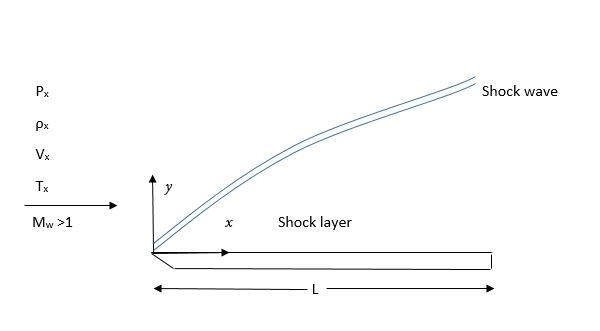
\includegraphics[scale=0.6]{images/Supersonic_flow_over_a_sharp_leading_edged_flat_plate_at_zero_incidence.png} 
		\caption{Supersonic flow over an infinitely thin flat plate, from Wikimedia Commons [2014].}
		\label{fig:wikimedia_flatPlate}
	\end{center}
\end{figure}




\begin{figure}[!htb]
	\begin{center}
		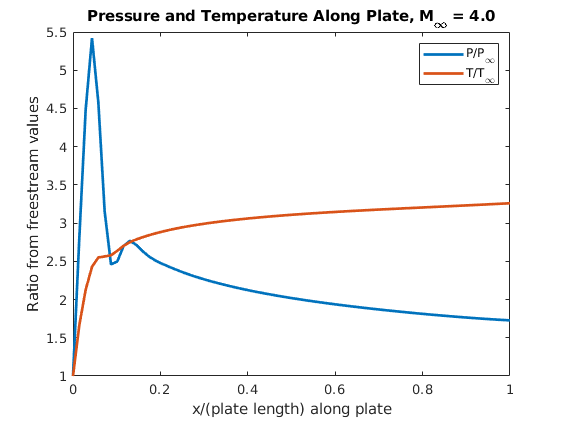
\includegraphics[scale=0.7]{images/UpperFlatPlate_PresTemp.png} 
		\caption{Pressure and Temperature ratio along the surface of the plate, where inflow is coming from the left and outflow to the right.}
		\label{fig:UpperFlatPlate_PresTemp}
	\end{center}
\end{figure}

\begin{figure}[!htb]
	\begin{center}
		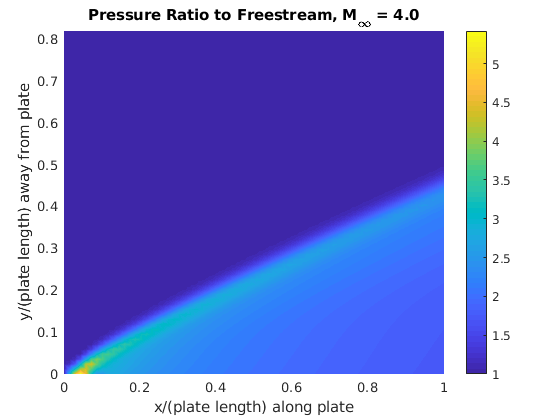
\includegraphics[scale=0.7]{images/UpperFlatPlate_PresMap.png} 
		\caption{Contour of $p/p_{atm}$ over the entire grid, with freestream flow moving from the left boundary to right and the flat plate fixed to the bottom boundary. The shockwave is visibe in lighter colors, compared to the dark blue being freestream conditions.}
		\label{fig:UpperFlatPlate_PresMap}
	\end{center}
\end{figure}

\begin{figure}[!htb]
	\begin{center}
		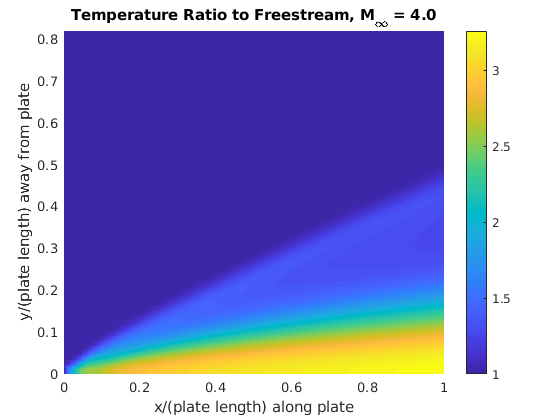
\includegraphics[scale=0.7]{images/UpperFlatPlate_TempMap.png} 
		\caption{Contour of $T/T_{atm}$ over the entire grid, with freestream flow moving from the left boundary to the right and the flat plate fixed to the bottom boundary. The shockwave is visible in lighter colors, compared to the dark blue being freestream conditions.}
		\label{fig:UpperFlatPlate_TempMap}
	\end{center}
\end{figure}

\begin{figure}[!htb]
	\begin{center}
		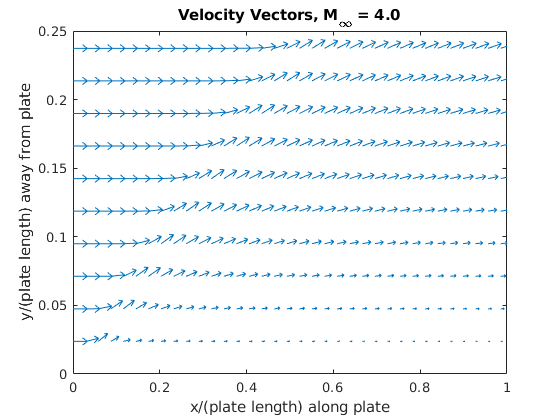
\includegraphics[scale=0.7]{images/UpperFlatPlate_VelocityVectors.png} 
		\caption{Quiver plot of the $u$ and $v$ velocities at each point, zoomed in around the bottom boundary to highlight the velocities through the shockwave.}
		\label{fig:UpperFlatPlate_VelocityVectors}
	\end{center}
\end{figure}


\FloatBarrier



\subsection*{Flow Over Upper and Lower Surfaces}


Compared to the first case where only the upper surface was calculated, what if now both the top and bottom are considered simultaneously? This is a simple extension to the above code, with only small changes being made to the boundary conditions, and the grid being doubled in size in the y-direction.\\

Compared to before where the plate was at the lower boundary, it is now moved to the center of the grid in the y-direction. The bottom boundary condition now receives the same conditions as the inflow and top, in that $v$ is enforced to be zero, and the other parameters are set to freestream conditions. At the "infinitely thin" plate, two cells in the vertical direction need to be allocated in order to track the pressure and temperature at the top and bottom surfaces independently. The $u$ and $v$ velocity are both set to zero on the plate as before to enforce the no-slip condition.\\

First lets examine flow around the plate at zero angle of attack, as seen below.\\

In Figure~\ref{fig:TwoPlate_PresTemp_0AoA} the pressure and temperature profiles for the upper and lower portions of the plate; as the system is symmetrical, we expect the profiles to be identical which they appear to be.\\

In Figures~\ref{fig:TwoPlate_PresMap_0AoA} through \ref{fig:TwoPlate_VelocityVectors_0AoA} the flow is further visualized and the solution over the lower plate appears to be symmetrical with that over the upper plate.\\

\FloatBarrier

\begin{figure}[!htb]
	\begin{center}
		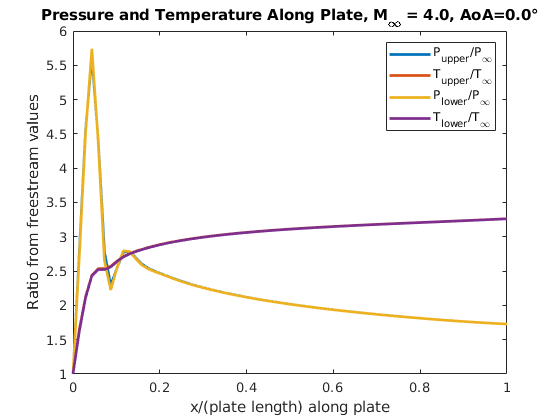
\includegraphics[scale=0.7]{images/TwoPlate_PresTemp_0AoA.png} 
		\caption{Pressure and Temperature ratio along the surface of the plate, where inflow is coming from the left and outflow to the right.}
		\label{fig:TwoPlate_PresTemp_0AoA}
	\end{center}
\end{figure}

\begin{figure}[!htb]
	\begin{center}
		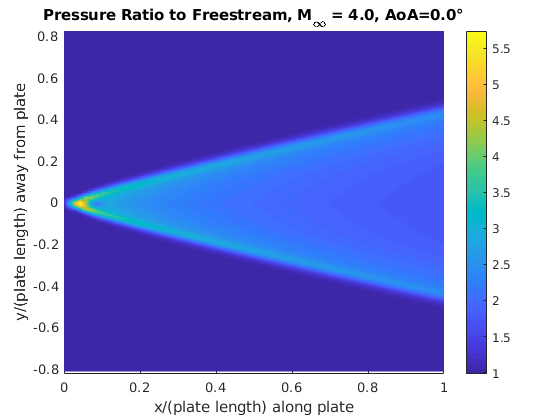
\includegraphics[scale=0.7]{images/TwoPlate_PresMap_0AoA.png} 
		\caption{Contour of $p/p_{atm}$ over the entire grid, with freestream flow moving from the left boundary to right and the flat plate fixed to the bottom boundary. The shockwave is visibe in lighter colors, compared to the dark blue being freestream conditions.}
		\label{fig:TwoPlate_PresMap_0AoA}
	\end{center}
\end{figure}

\begin{figure}[!htb]
	\begin{center}
		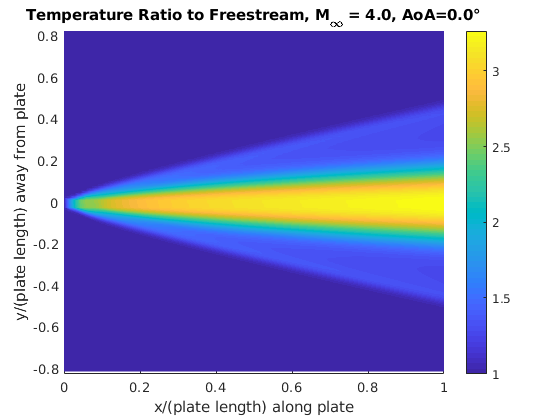
\includegraphics[scale=0.7]{images/TwoPlate_TempMap_0AoA.png} 
		\caption{Contour of $T/T_{atm}$ over the entire grid, with freestream flow moving from the left boundary to the right and the flat plate fixed to the bottom boundary. The shockwave is visible in lighter colors, compared to the dark blue being freestream conditions.}
		\label{fig:TwoPlate_TempMap_0AoA}
	\end{center}
\end{figure}

\begin{figure}[!htb]
	\begin{center}
		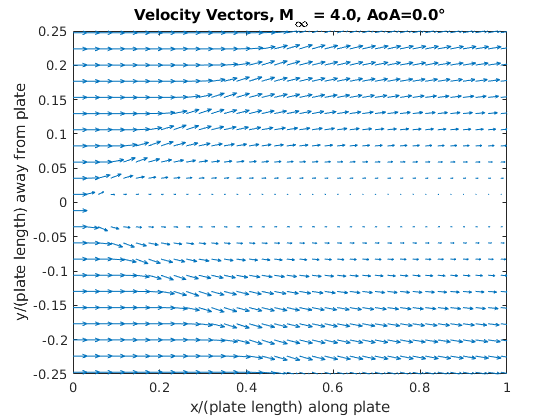
\includegraphics[scale=0.7]{images/TwoPlate_VelocityVectors_0AoA.png} 
		\caption{Quiver plot of the $u$ and $v$ velocities at each point, zoomed in around the bottom boundary to highlight the velocities through the shockwave.}
		\label{fig:TwoPlate_VelocityVectors_0AoA}
	\end{center}
\end{figure}

\FloatBarrier


But now how does the flow change when the plate is set at an angle of attack, rather than zero incident angle? This is applied by setting a non-zero value for the $v$ velocity at the left and bottom (inflow) boundaries, where:

\begin{align*}
v = u \tan (\alpha)
\end{align*}

for angle of attack $\alpha$.\\

This flow profile is seen below in Figure~\ref{fig:TwoPlate_PresMap_Combined}, where as the angle of attack increases, the shockwave becomes less linear and the maximum pressure at the leading edge increases significantly.


\FloatBarrier

\begin{figure}[!htb]
	\begin{center}
		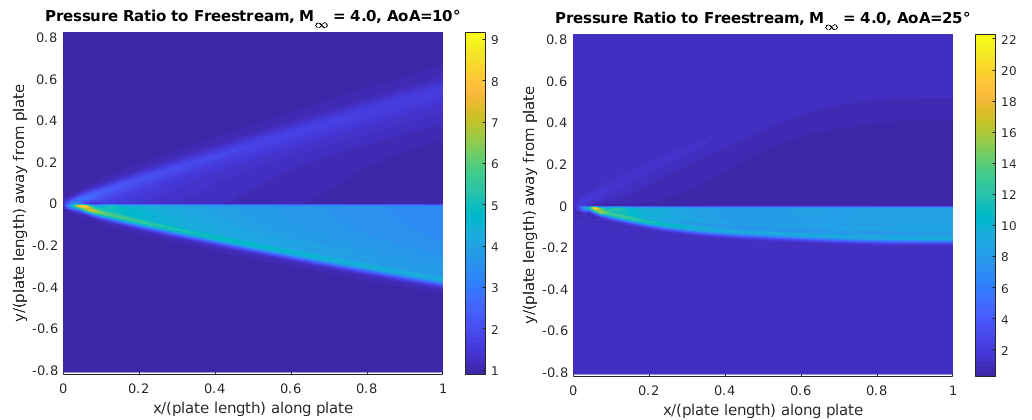
\includegraphics[scale=0.45]{images/TwoPlate_PresMap_Combined.png} 
		\caption{Contour of $p/p_{atm}$ over the entire grid for angle of attack at 10 degrees on the left, and angle of attack of 25 degrees on the right. At higher angles of attack, the $v$ velocity begins to deform the shockwave, and the maximum pressure becomes much higher at the leading edge.}
		\label{fig:TwoPlate_PresMap_Combined}
	\end{center}
\end{figure}



\begin{figure}[!htb]
	\begin{center}
		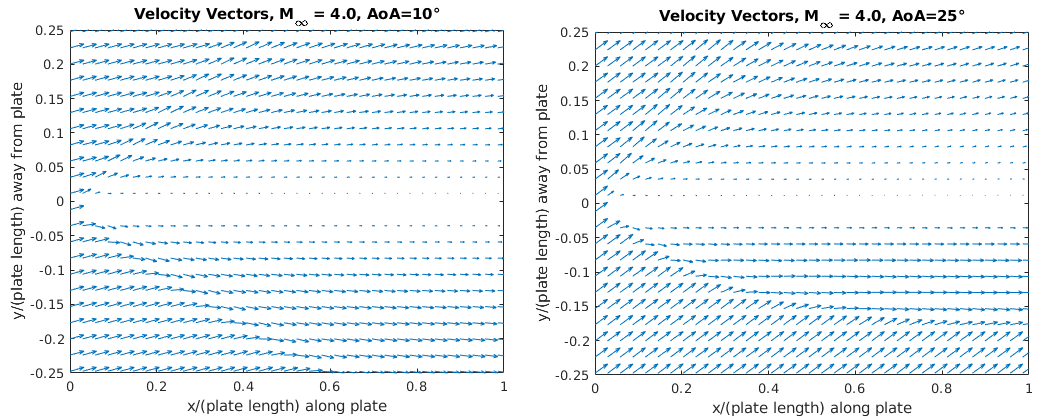
\includegraphics[scale=0.45]{images/TwoPlate_VelocityVectors_Combined.png} 
		\caption{Quiver plot of the $u$ and $v$ velocities at each point, zoomed in around the plate boundaries to highlight the velocities through the shockwave.}
		\label{fig:TwoPlate_VelocityVectors_Combined}
	\end{center}
\end{figure}


\FloatBarrier

As the angle of attack is increased the temperature profiles in Figure~\ref{fig:TwoPlate_PresTemp_10AoA} remain similar, but the pressure values quickly diverge with the pressure under the plate being greater than that on top of the plate. This is what creates lift!\\

Integrating the pressure along the top and bottom of the plate and taking the difference, a lift per unit length (into the page) can be calculated, as shown below in Figure~\ref{fig:TwoPlate_Lift}.




\begin{figure}[!htb]
	\begin{center}
		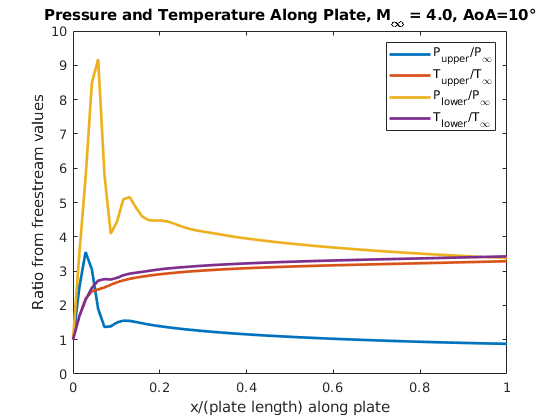
\includegraphics[scale=0.7]{images/TwoPlate_PresTemp_10AoA.png} 
		\caption{Pressure and temperature ratios along the upper and lower surface of the plate. As the angle of attack is increased, the pressure along the upper side decreases and the lower side increases, causing the creation of lift.}
		\label{fig:TwoPlate_PresTemp_10AoA}
	\end{center}
\end{figure}




\begin{figure}[!htb]
	\begin{center}
		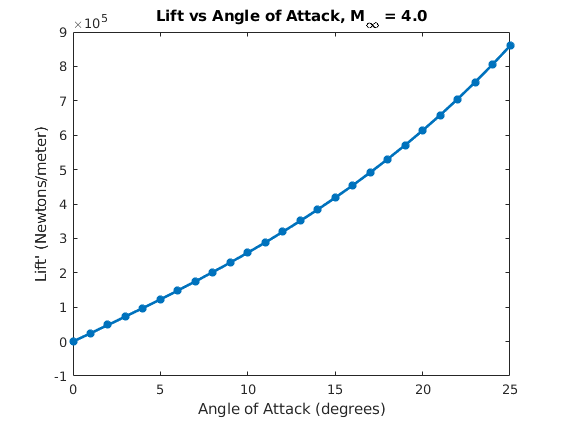
\includegraphics[scale=0.7]{images/LiftVSAoA.png} 
		\caption{Calculation of lift per unit length (into the page) for a flat plate at 0 to 25 degrees angle of attack. Symmetric airfoils (or in this case infinitely thin flat plates,) do not create lift at zero angle of attack. Airfoil camber is introduced to change this.}
		\label{fig:TwoPlate_Lift}
	\end{center}
\end{figure}




\FloatBarrier



% first show just our base code with the shockwave over the top 

% then the top and bottom version with 0 incident angle

% then at some non-zero incident angle

% potentially we can calculate lift vs incident angle at different incoming velocities?
% like M=0.5, 1.0, 2.0, 4.0


\section*{APPLICATION: Couette Flow}

% go over boundary conditions, where's a wall vs fixed vs free values

Couette flow describes the flow between two flat plates, where one is stationary and the other is moving with some constant velocity. For initial conditions, it is assumed that the fluid within the channel starts at zero velocity in both x and y directions at time zero, and the upper wall is started instantaneously to it's nominal velocity. The inflow and outflow boundaries are both allowed to move freely and are interpolated from the flow interior. The no slip condition is enforced along both walls.\\

The velocity profile at the center (away from inflow and outflow) is shown below in Figure~\ref{fig:CouetteFlowStartup} through time, and depicts the flow going from zero velocity up to a linear decrease across the channel between the moving and stationary plates.\\



\FloatBarrier

\begin{figure}[!htb]
	\begin{center}
		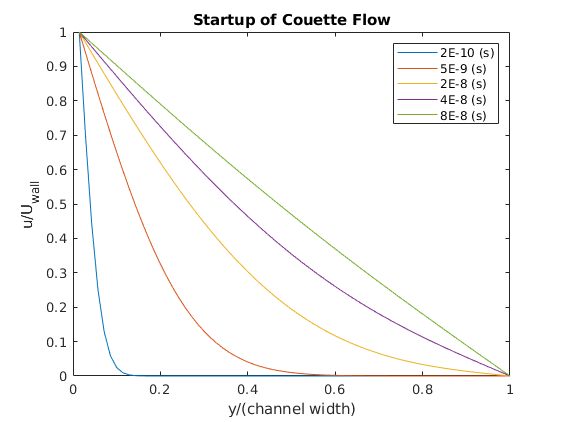
\includegraphics[scale=0.7]{images/FlowStartup.png} 
		\caption{Velocity profile of channel flow from start to steady state. $U_{wall}$ was set to 100 m/s and Channel Width $10^{-5}$m to allow for faster convergence.}
		\label{fig:CouetteFlowStartup}
	\end{center}
\end{figure}


\FloatBarrier


While the above case depicts how the flow develops under a zero pressure gradient, a pressure gradient is often present and can further increase or decrease the flow depending on if the pressure gradient is in the same direction as the moving plate or the opposite.\\

Figure~\ref{fig:Couette_decreasingPres} depicts the case of a negative pressure gradient, where the inflow boundary pressure was set to 1.25atm and the outflow 1.00atm; this pressure gives the flow an extra "push" down the pipe and we see the velocities increase above that of the wall speed. \\

For Figure~\ref{fig:Couette_increasingPres} the inflow and outflow pressures were switched between 1.00atm and 1.25atm respectively. Now the pressure gradient is working against the moving wall and an overall decrease is seen, with flow closer to the stationary wall reversing direction and moving back towards the inflow boundary (which was left as free.)\\

Both of these results are as expected for idealized flow.\\




\begin{figure}[!htb]
	\begin{center}
		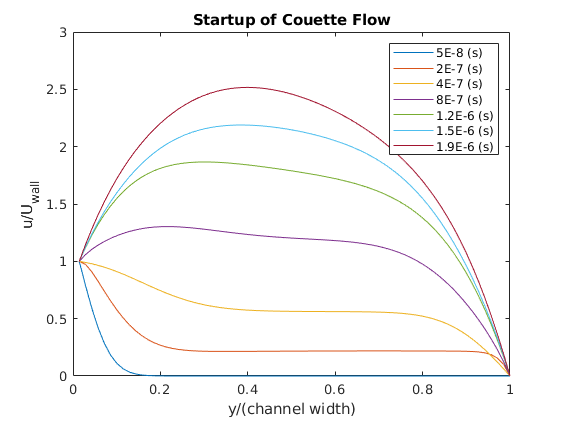
\includegraphics[scale=0.7]{images/FlowStartup_DecreasingPressure.png} 
		\caption{Velocity profile of channel flow from start to steady state, where inflow pressure was 1.25atm and outflow pressure 1.00atm. $U_{wall}$ was set to 100 m/s and Channel Width $10^{-5}$m to allow for faster convergence.}
		\label{fig:Couette_decreasingPres}
	\end{center}
\end{figure}


\begin{figure}[!htb]
	\begin{center}
		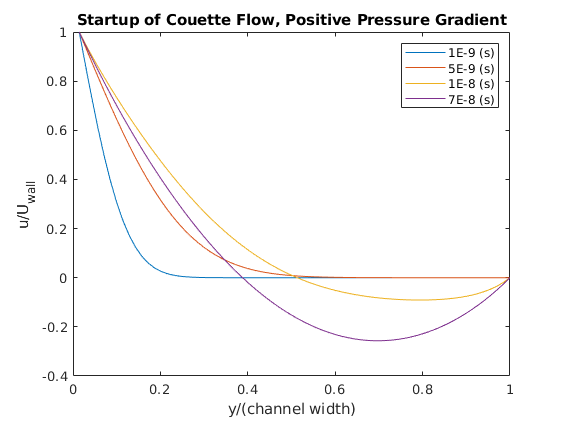
\includegraphics[scale=0.7]{images/FlowStartup_IncreasingPressure.png} 
		\caption{Velocity profile of channel flow from start to steady state, where inflow pressure was 1.00atm and outflow pressure 1.25atm. $U_{wall}$ was set to 100 m/s and Channel Width $10^{-5}$m to allow for faster convergence.}
		\label{fig:Couette_increasingPres}
	\end{center}
\end{figure}



% zero pressure gradient
% positive pressure gradient
% negative pressure gradient



\FloatBarrier


\renewcommand\refname{REFERENCES}

\begin{thebibliography}{9}
	\bibitem{Anderson} 
	Anderson
	\textit{Computational Fluid Dynamics: The Basics with Applications}. 
	McGraw-Hill, 1995
	
	\bibitem{MacCormack2dNotes}
	Baeder
	\textit{MacCormack 2D Notes}.
	
	\bibitem{wikimedia_flatPlate}
	Silawat
	\textit{Supersonic flow over a sharp leading edged flat plate at zero incidence}
	\url{https://commons.wikimedia.org/wiki/File:Supersonic_flow_over_a_sharp_leading_edged_flat_plate_at_zero_incidence.JPG}

	
	
\end{thebibliography}



\section*{CODE}

Attached is the base code written in both CUDA C and then MATLAB. Small changes to plate location, initial flow conditions, and boundary conditions were made to the MATLAB version create each of the above cases. 

\subsection*{NavierStokesSolver.cu}
\lstinputlisting{code/NavierStokesSolver.cu}



\subsection*{initialize.m}
\lstinputlisting{code/initialize.m}

\subsection*{BoundaryLayerThickness.m}
\lstinputlisting{code/BoundaryLayerThickness.m}

\subsection*{calc\_dt.m}
\lstinputlisting{code/calc_dt.m}

\subsection*{calc\_Q.m}
\lstinputlisting{code/calc_Q.m}

\subsection*{calc\_FG.m}
\lstinputlisting{code/calc_FG.m}

\subsection*{heatFluxParameters.m}
\lstinputlisting{code/heatFluxParameters.m}

\subsection*{shearParameters.m}
\lstinputlisting{code/shearParameters.m}

\subsection*{MaccormackPredictorUniform.m}
\lstinputlisting{code/MaccormackPredictorUniform.m}

\subsection*{primativesFromQ.m}
\lstinputlisting{code/primativesFromQ.m}

\subsection*{enforceBC\_nonSurface.m}
\lstinputlisting{code/enforceBC_nonSurface.m}

\subsection*{enforceBC\_surface.m}
\lstinputlisting{code/enforceBC_surface.m}

\subsection*{MaccormackCorrectorUniform.m}
\lstinputlisting{code/MaccormackCorrectorUniform.m}




%\subsection*{ENAE685\_HW7}
%\lstinputlisting{code/ENAE685_HW7.m}
%
%\subsection*{ic\_switch()}
%\lstinputlisting{code/ic_switch.m}
%
%\subsection*{init()}
%\lstinputlisting{code/init.m}
%
%\subsection*{prim\_to\_cons()}
%\lstinputlisting{code/prim_to_cons.m}
%
%\subsection*{flux()}
%\lstinputlisting{code/flux.m}
%
%\subsection*{calc\_dt()}
%\lstinputlisting{code/calc_dt.m}
%
%\subsection*{cons\_to\_prim()}
%\lstinputlisting{code/cons_to_prim.m}
%
%\subsection*{exact\_euler()}
%\lstinputlisting{code/exact_euler.m}
%
%\subsection*{errorcalc()}
%\lstinputlisting{code/errorcalc.m}


\end{document}